\section{An Analysis of Feature Regularization}
We briefly introduce the notations in our work: we denote uppercase $A$, bold $\mathbf{a}$ and lowercase $a$ for matrices, vectors and scalars respectively. For a vector $\mathbf{a}_i$, we denotes $\mathbf{a}_{i,j} $ as its $j$-th element.  $||.||_F$ stands for the Frobenius norm of a matrix. Given $N$ examples $\{(\mathbf{x}^i,y^i)|i=1,...,N\}$, we define $\mathbb{E}\{.\}$ as an expectation taken with respect to the empirical distribution generated by the training set.

Following \cite{low-shot}, we aim to learn a neural network model to extract the  feature representations $\phi(\mathbf{x}^i)$ and make predictions $\hat{y}_i=W\phi(\mathbf{x}^i)$ with $W=[\mathbf{w}_1,...,\mathbf{w}_{|C|}]$. This setting includes both classification and regression problems, with $|C|$ as the number of classes or target dimension, respectively. The problem can be generally formulated as:
\begin{equation}
W^*,\phi^*=\arg\min_{W,\phi}\mathbb{E}\{l(W,\phi(\mathbf{x}^i),y^i)\}
\end{equation}
where $l(.)$ can be any reasonable cost function. {\color{red}In this paper, we focus on cross-entropy and  $L_2$ loss due to their convexity and universality.} % Specifically, if $l(.)$ a metric learning loss as in \cite{one-shot-siamese,low-shot}, $W$ is empty and we only optimize $\phi(.)$.% This can be generally optimized with an online stochastic gradient descent (SGD).

In \cite{low-shot}, it is suggested that adding a squared gradient magnitude loss (SGM) on every sample can regularize the learning process.
\begin{equation}
W^*,\phi^*=\arg\min_{W,\phi}\mathbb{E}\{l(W,\phi(\mathbf{x}^i),y^i)+\lambda||\nabla_Wl(W,\phi(\mathbf{x}^i,y^i))||^2\}
\end{equation}
The insight is that for a good solution, the parameter gradient should be small at convergence. However, we know that the convergence of a neural network optimization is a dynamic equilibrium. In other words, at a stationary point, we should have $\mathbb{E}\{\nabla_W l(W,\phi(\mathbf{x}))\}\rightarrow0$. Intuitively %As pointed out in \cite{big-data}, 
when close to convergence, about half of the data-cases recommend to update a parameter to move {\color{red}positive}, while the other half recommend to move {\color{red}negative}. It is not very clear why \textit{small gradients on every sample} $\mathbb{E}\{||\nabla_W l(W,\phi(\mathbf{x}))||^2\}$ produces good generalization experimentally.

Mathematical derivation shows that the optimization problem with gradient penalty is equivalent with adding a weighted $L_2$ regularizer $\phi(\mathbf{x}^i)$:
\begin{eqnarray}
\arg\min_{W,\phi}\mathbb{E}\{l(W,\phi(\mathbf{x}^i),y^i)+\lambda\alpha^i||\phi(\mathbf{x}^i)||^2\}
\label{eqn:cost}
\end{eqnarray}
where the example-dependent $\alpha^i$ measures the deviation between the prediction $\hat{y}^i$ and the target $y^i$.  %$\alpha^i$ is higher for examples that are misclassified, and nears zero for correct ones. 
In a regression problem, we have $\alpha^i=r^2=||\hat{y}^i-y^i||^2$, with the residual $r=\hat{y}^i-y^i$; in a classification problem, we have $\alpha^i=\sum_k(p^i_k-I(y^i=k))^2$. Intuitively, the misclassified high-norm examples might be outliers, and in a low-shot learning scenario, such outliers can pull the learned weight vectors far away from the right solution. In \cite{low-shot}, the authors compare dropping $\alpha^i$ and directly penalizing $||\phi(x^i)||^2$, which performs almost equally well. %experimentally. 

In our work, we argue that a better and more reasonable design should be:
\begin{eqnarray}
\arg\min_{W,\phi}\mathbb{E}\{l(W,\phi(\mathbf{x}^i),y^i)+\lambda_1\alpha^i||\phi(\mathbf{x}^i)||^2\}+\lambda_2||W||_F^2
\label{eqn:final-cost}
\end{eqnarray}
where we add another weight regularizer $||W||_F^2$, which is necessary to avoid degenerate solutions. We will give further explanation in our second case study. In following analysis, we denote the cost in Eqn(\ref{eqn:final-cost}) with example-dependent $\alpha^i$ as \textit{\textbf{weighted $L_2$ feature penalty}}, and the example-independent (setting $\alpha^i\equiv1$) as \textit{\textbf{uniform $L_2$ feature penalty}}. % We will analyze in the following section (case study 2) why the final weight $||W||_F^2$ is necessary.

% However, the $L_1$ regularization achieves inferior performance.
We carry out two case studies: (1) an XOR classification and (2) a regression problem, both empirically and theoretically to analyze how the uniform and weighted $L_2$ feature penalty regularize the neural network. In our paper, we will focus on the \textit{\textbf{uniform}} feature regularization and will also cover the \textit{\textbf{weighted}} scenario as well.




\subsection{Case Study 1: an Empirical Analysis of XOR Classification}
\label{sec:empirical}
First, we study the simplest linear-non-separable problem-- exclusive-or (XOR). Suppose that we have four two-dimensional input points $\mathbf{x}=[x_1,x_2]^T\in R^2$: $\{\mathbf{x}^1=[1,1]^T,\mathbf{x}^2=[0,0]^T\}\in C_+$ belongs to the positive class, while $\{\mathbf{x}^3=[1,0]^T,\mathbf{x}^4=[0,1]^T\}\in C_-$ the negative. 

As shown in Figure \ref{fig-xor}, we use a three-layer neural network to address the problem (left figure): $\mathbf{h_1}=\mathbf{x}+\mathbf{b}$ is a translation with  $\mathbf{b}=[b_1,b_2]^T\in R^2$ as the offset; $h_2=h_{1,1}*h_{1,2}$ is a non-linear layer, multiplying the first and second dimension of $\mathbf{h}_1$ and producing a scalar; $y$ is a linear classifier on $h_2$ parametrized by $w$. The original classification problem can be formulated as:
\begin{eqnarray*}
\arg\min_{w_1,\mathbf{b},w}\sum_{i=1}^4\log(1+\exp(-y^i*w*h^i_2))
%\label{eqn:final-cost}
\end{eqnarray*}

Suppose that we start from an initialization $\mathbf{b}=[0,0]^T$, all three samples $\{\mathbf{x}^2,\mathbf{x}^3,\mathbf{x}^4\}$ from different classes will produce the same representation $h_2=0$, which is not separable at all. It takes efforts to tune the learning rate to back-propagate $w,\mathbf{b}$ updates from the target $y$.

However, if we introduce the \textit{\textbf{uniform}} $L_2$ feature regularization as:
\begin{eqnarray*}
\arg\min_{w_1,\mathbf{b},w}\sum_{i=1}^4\log(1+\exp(-y^iwh^i_2))+\frac{\lambda_1}{2}||h^i_2||^2%+\lambda_2||w||^2
\end{eqnarray*}
Then, we have:
\begin{eqnarray}
\frac{\lambda_1}{2}\frac{\partial ||h_2||^2}{\partial\mathbf{b}}=\lambda_1
\binom{\mathbb{E}\{h_2(x_2+b_2)\}} {\mathbb{E}\{h_1(x_1+b_1)\}}
\label{eqn:xor-reg}
\end{eqnarray}
the gradient descent pulls Eqn(\ref{eqn:xor-reg}) towards zero, i.e., pulling $\mathbf{b}$ towards $b_1=-\mathbb{E}\{x_1\}=-0.5$ and $b_2=-\mathbb{E}\{x_2\}=-0.5$.
\begin{figure}
	\begin{center}
		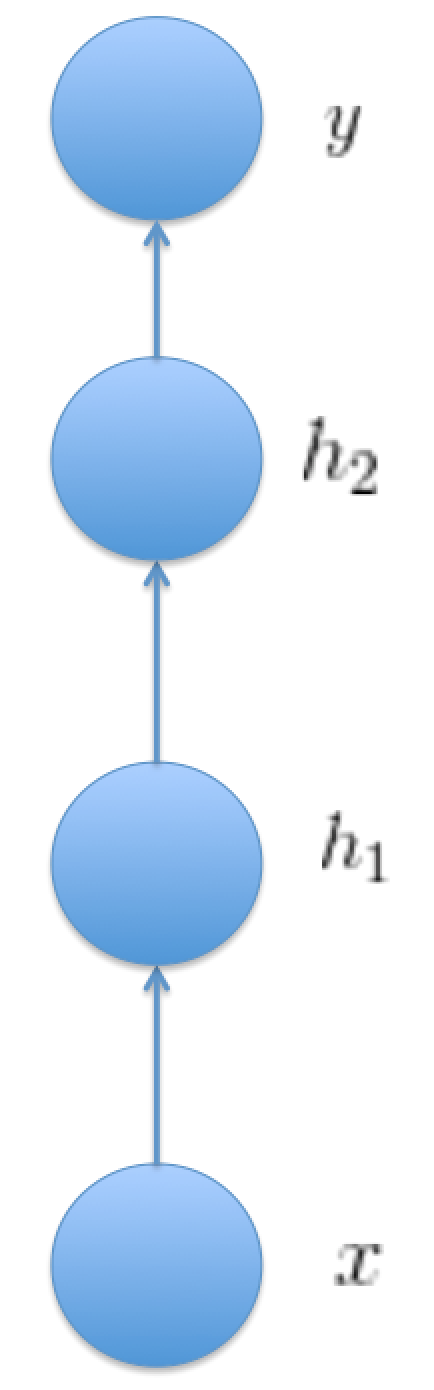
\includegraphics[width=0.1\columnwidth]{xor.png}
		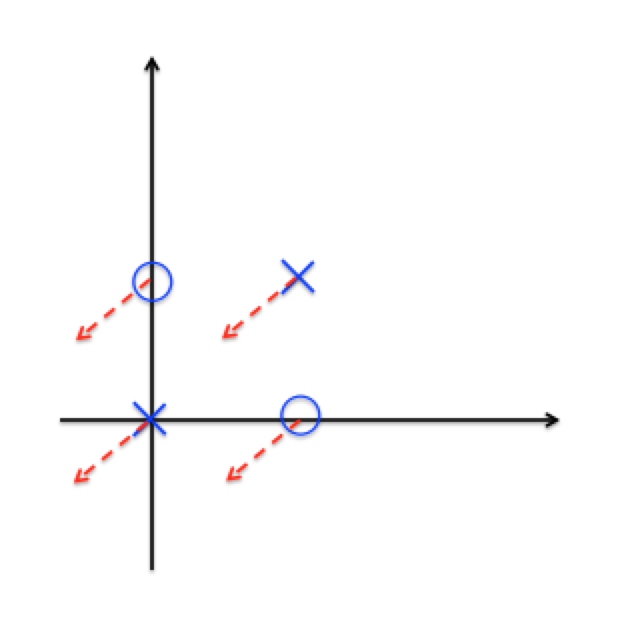
\includegraphics[width=0.35\columnwidth]{xor-analysis.png}
		%
		%	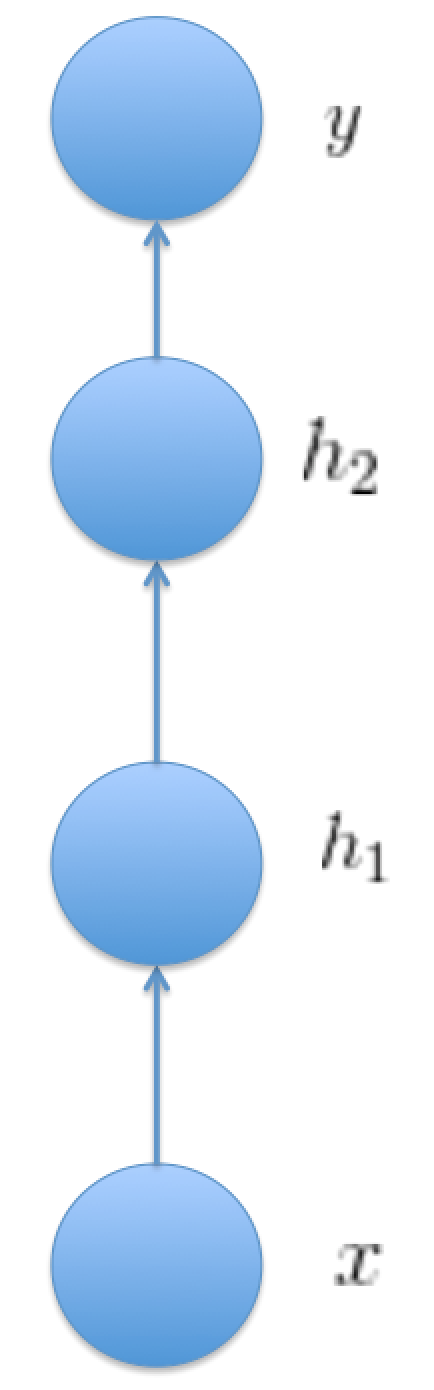
\includegraphics[width=0.3\columnwidth]{xor.png}\hspace{+0.5mm}
		%	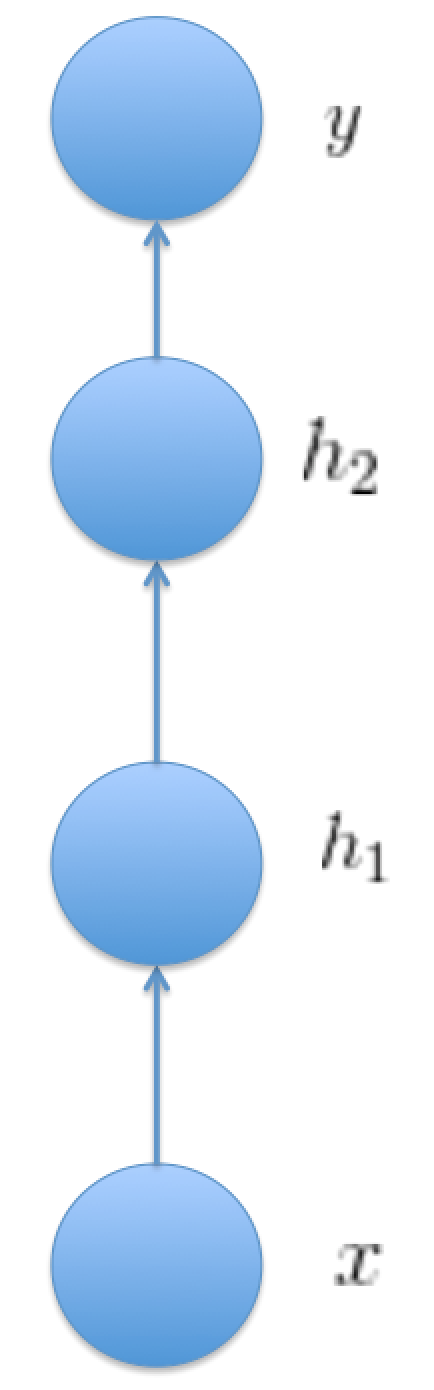
\includegraphics[width=0.3\columnwidth]{xor.png}\vspace{+1mm}\\
		%\end{center}
		%\hspace{+0mm}
		%\vspace{-2mm}
	\end{center}
	\caption{Case 1: an empirical study of the XOR classification task. {\bf The left figure:} the network structure we use: $h_1$ is a linear transformation, $h_2$ is a non-linear transform of $h_1$ and $y$ is the prediction; {\bf The right column:} The linear transformation maps $\mathbf{x}$ to $\mathbf{h_1}$. As shown in the red arrow, an $L_2$ norm penalty on $h_2$ centers the feature of $h_1$ and make the points from different sets separable. 'X's refer to positive examples, and 'O's are negative ones.}
	\label{fig-xor}
\end{figure}

%We can easily observe that the choice of $w,\mathbf{b}$ is critical to make the following feature $h_2$ trainable.  
As shown on the right of Figure \ref{fig-xor}, the gradient of feature regularization
pulls $\mathbf{h_1}$ along the direction of red arrows. Then, we have $h_2>0$ for positive examples and $h_2<0$ for negative ones, which means $h_2$ is linearly-separable. In summary, we can observe that:\\
\textbf{Empirically, the feature regularization \textit{centers} the representation $h_2=\phi(\mathbf{x})$ and makes the following classification more learnable}.\\
For the weighted case, the offset $\mathbf{b}$ have similar effects. It can be derived that when converged the feature representation will satisfy $\mathbb{E}\{\mathbf{h}_1\}=\mathbf{0}$ and $\mathbb{E}\{h_2\}$=0.

\begin{figure}
	\begin{center}
		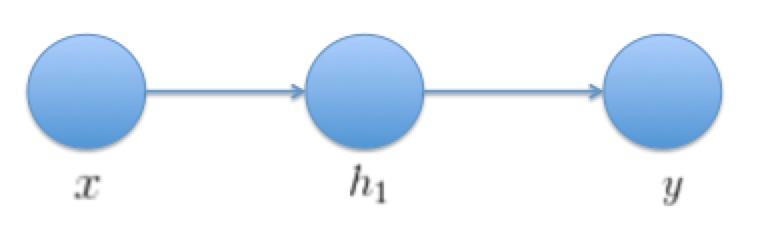
\includegraphics[width=0.35\columnwidth]{regression.png}
	\end{center}
	%\begin{center}
	%	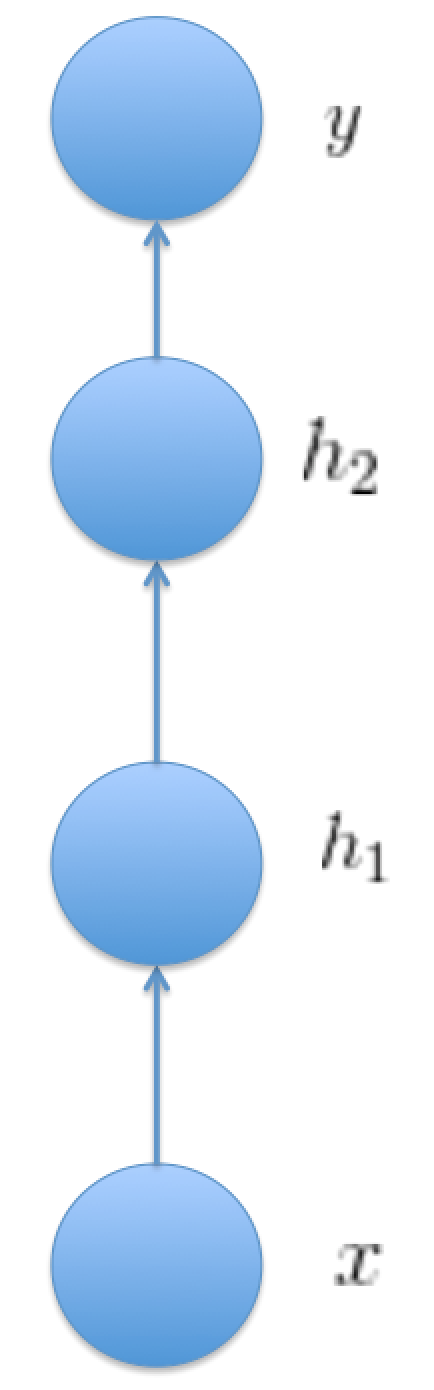
\includegraphics[width=0.3\columnwidth]{xor.png}\hspace{+0.5mm}
	%	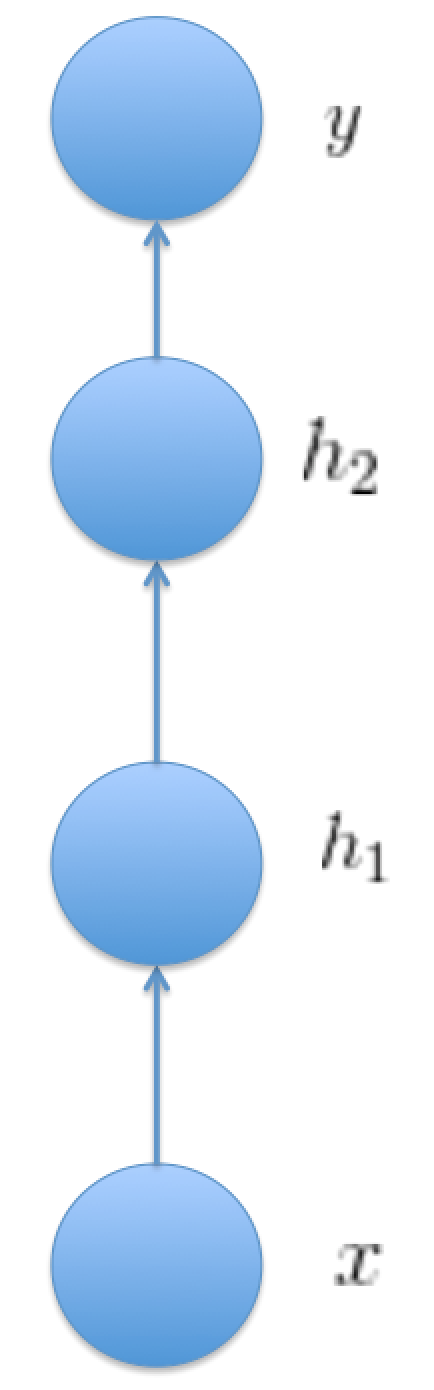
\includegraphics[width=0.3\columnwidth]{xor.png}\vspace{+1mm}\\
	%\end{center}
	%\hspace{+0mm}
	%\vspace{-2mm}
	\caption{Case 2: a comprehensive study of a two-layer linear neural network for regression task. We minimize the $L_2$ distance between the prediction $\hat{y}=W_2(W_1\mathbf{x}+\mathbf{b}_1)+\mathbf{b}_2$ and $y$. The latent representation $\mathbf{h}=W_1\mathbf{x}+b_1$ is a linear mapping.}
	\label{fig-regression}
\end{figure}
\subsection{Case Study 2: a Comprehensive Analysis on a Regression Problem}
Next, we analyze a two-layer linear neural network as shown in Figure \ref{fig-regression}. Denoting the input as $X=[\mathbf{x}_1,\mathbf{x}_2,...]$ and the target as $Y=[\mathbf{y}_1,\mathbf{y}_2,...]$. The regression loss can be formulated as:
\begin{eqnarray*}
\mathbf{E}\{||y-W_2W_1x||^2\} 
\end{eqnarray*}
where the latent feature is $\mathbf{h}=\phi(\mathbf{x})=W_1\mathbf{x}$. The optimization of $\{W_1,W_2\}$ in this multi-layer linear neural network is not trivial, since it satisfies following properties:
\begin{enumerate}
\item The regression loss is non-convex and non-concave. It is convex on $W_1$ (or $W_2$) when the other parameter $W_2$ (or $W_1$) is fixed, but not convex on both simultaneously;
\item Every local minimum is a global minimum;
\item Every critical point that is not a global minimum is a saddle point;
\item If $W_2*W_1$ is full-rank, the Hessian at any saddle point has at least one negative eigenvalue.
\end{enumerate}
We refer interested readers to \cite{nn-global-minima,deep-global-minima} for detailed analysis. 

In case of the uniform $L_2$ feature penalty, the problem becomes:
\begin{equation}
E(W_1,W_2)=\mathbb{E}\{\frac{1}{2}||\mathbf{y}-W_2W_1\mathbf{x}||^2+\frac{\lambda_1}{2}||W_1\mathbf{x}||^2\}+\frac{\lambda_2}{2}||W_2||_F^2
\end{equation}
At the global minimum $\{W_1^*,W_2^*\}$, we should have:
\begin{eqnarray}
\frac{\partial E}{\partial W_1}|_{W_1^*}=W^T_2\Sigma_{xy}-W^T_2W_2W_1\Sigma_{xx}
+\lambda_1W_1\Sigma_{xx}=0\\
\frac{\partial E}{\partial W_2}|_{W_2^*}=\Sigma_{xy}W_1^T-W_2W_1\Sigma_{xx}W_1^T+\lambda_2W_2=0
\end{eqnarray}
where we define the variance and covariance matrix as $\Sigma_{xx}=\mathbb{E}\{\mathbf{x}\mathbf{x}^T\}$, $\Sigma_{xy}=\mathbb{E}\{\mathbf{y}\mathbf{x}^T\}$.
Carrying out $Eqn(7)*W_1^T-W_2^T*Eqn(8)=0$ reveals a very interesting conclusion:
\begin{equation}
\lambda_1\mathbb{E}\{||W_1\mathbf{x}||^2\}=\lambda_2||W_2||_F^2
\label{eqn:equal-energy}
\end{equation}
This reads as \textit{\textbf{the expected $L_2$ feature penalty should be equal to final-layer weight regularizer when converged}}. Or equivalently, when close to convergence, the $L_2$ feature penalty reduces over-fitting by implicitly penalizing the corresponding weight matrix $W$. A more generalized form is:
\newtheorem{theorem}{Lemma}
\begin{theorem}
For a cost function of form in Eqn (\ref{eqn:final-cost}) with uniform $L_2$ feature regularization:
\begin{eqnarray*}
\arg\min_{W,\phi}\mathbb{E}\{l(W,\phi(\mathbf{x}^i),y^i)+\lambda_1||\phi(x_i))||^2\}+\lambda_2||W||_F^2
\end{eqnarray*}
we have:
\begin{equation}
\lambda_1\mathbb{E}\{||\phi(\mathbf{x})||^2\}=\lambda_2||W||_F^2
\end{equation}
\end{theorem}
The $\phi(.)$ can take a quite general form of a convolutional neural network with many common non-linear operations such as the ReLU, max-pooling and so on. One can follow the derivation of Eqn(\ref{eqn:equal-energy}) to easily derive \textbf{Lemma 1}.

Lemma 1 also reveals the importance of adding the weight penalty $||W||^2_F$ in Eqn(\ref{eqn:final-cost}). If we only include the the feature penalty and drop the weight penalty ($\lambda_2=0$ in our case), then a scaling as $\phi(.)=\gamma\phi(.)$ and $W=\frac{1}{\gamma}W$ with $\gamma<1$ will always decrease the energy and the solution will become very ill-conditioned with $\gamma\rightarrow 0$.
\subsubsection{$L_2$ Feature Regularization Makes Optimization Easier}
Moreover, we analyze numerically how the $L_2$ feature penalty influences the optimization process in our regression problem. % Here, we analyze both the \textit{\textbf{uniform}} and \textit{\textbf{weighted}} $L_2$ feature penalty scenario.

We study a special case $\{\mathbf{x}\in\mathbb{R}^d,y\in\mathbb{R}\}$ with $W_1\in\mathbb{R}^{1\times m}$, $W_2\in\mathbb{R}$ and include offsets $b_1\in\mathbb{R}$ and $b_2\in\mathbb{R}$ to make the problem more general. Then, the latent representation becomes $h=W_1\mathbf{x}+\mathbf{b}_1$ and the prediction is $\hat{y}=W_2h+b_2$. The cost function of Eqn(\ref{eqn:final-cost}) becomes:
%By dropping $\alpha_i$ in Eqn (3), we show that $L_2$ feature penalty actually regularizes the representation similar to a soft batch normalization. Here, we analyze the numerical behavior with $\alpha_i$ remaining.
\begin{equation}
E(W_1,b_1,W_2,b_2)=\frac{1}{2}\mathbb{E}\{(W_2h+b_2-y)^2+\frac{\lambda_1}{2} r_{\dagger}^2h^2\}+\frac{\lambda_2}{2}W_2^2
\label{eqn:final-regression}
\end{equation}
We define the prediction residual $r$ and $r_{\dagger}$ as $\hat{y}-y$ for better readability, and substitute $\alpha^i=(r^i_{\dagger})^2$. 
%to avoid the degenerate case with very $\{\mathbf{w}_1,b_1\}\rightarrow\mathbf{0}$ and $w_2\rightarrow\infty$.
Numerically, we apply a \textbf{two-step} process: in the first step, we calculate the sample-dependent $r^i_{\dagger}$ in the feed-forward process to obtain our $L_2$ feature regularization weights $\alpha^i$ for each $(\mathbf{x}^i,y^i)$; in the second step, we treat $r_{\dagger}$ as a constant in the  optimize. 
%Then in the setting of online learning, 
The gradient and Hessian matrix of Eqn(\ref{eqn:final-regression}) can be derived as:
\begin{align*}
\frac{\partial E}{\partial W_2}&=\mathbb{E}\{rh^T\}+\lambda_2W_2 
&\frac{\partial E}{\partial b_2}&=\mathbb{E}\{r\}\\
\frac{\partial E}{\partial h^i}&=W_2r^i+\lambda_1(r^i_{\dagger})^2h^i\\
\frac{\partial E}{\partial W_1}&=W_2\mathbb{E}\{r\mathbf{x}^T\}+\lambda_1 \mathbb{E}\{r_{\dagger}^2h\mathbf{x}^T\}\\
\frac{\partial E}{\partial b_1}&=W_2\mathbb{E}\{r\}+\lambda_1 \mathbb{E}\{r_{\dagger}^2h\}
\end{align*}

\begin{comment}
\begin{align*}
\frac{\partial E}{\partial W_2}&=\mathbb{E}\{rh^T\}+\lambda_2W_2 
&\frac{\partial E}{\partial b_2}&=\mathbb{E}\{r\}
&\frac{\partial E}{\partial h^i}&=W_2r^i+\lambda_1(r^i_{\dagger})^2h^i\\
\frac{\partial E}{\partial W_1}&=W_2\mathbb{E}\{r\mathbf{x}^T\}+\lambda_1 \mathbb{E}\{r_{\dagger}^2h\mathbf{x}^T\}
&\frac{\partial E}{\partial b_1}&=W_2\mathbb{E}\{r\}+\lambda_1 \mathbb{E}\{r_{\dagger}^2h\}
\end{align*}
\end{comment}
and
\begin{align*}
\frac{\partial^2 E}{\partial W_2^2}&=\mathbb{E}\{hh^T\}+\lambda_2
&\frac{\partial^2 E}{\partial b_2^2}&=1\\
\frac{\partial^2 E}{\partial (h^i)^2}&=W_2^2+\lambda_1 (r^i_{\dagger})^2
&\frac{\partial^2 E}{\partial W_1^2}&=(W_2^2+\lambda_1 		\mathbb{E}\{r_{\dagger}^2\})\mathbb{E}\{\mathbf{x}\mathbf{x}^T\}\\
\frac{\partial^2 E}{\partial b_1^2}&=W_2^2+\lambda_1 \mathbb{E}\{r_{\dagger}^2\}
\end{align*}
Suppose that we apply a second-order optimization algorithm for the network parameter $\theta\in\{w_1,w_2,b_1,b_2\}$, the updates should be $\vartriangle\theta=-\eta*(\partial^2 E/\partial\theta^2)^{-1}(\partial E/\partial\theta)$ with $\eta>0$ as the step-size.
If we unluckily start from a bad initialization point $W_2\rightarrow0$, the updates of $h_i$, $W_1$ and $b_1$ are of the form:
\begin{eqnarray*}
\vartriangle h^i&=&-\eta(W_2^2+\lambda_1 (r^i_{\dagger})^2\})^{-1}(W_2r^i+\lambda_1(r^i_{\dagger})^2h^i)\\
	\vartriangle\mathbf{w}_1&=&-\eta[(W_2^2+\lambda_1\mathbb{E}\{ r_{\dagger}^2\})\mathbb{E}\{\mathbf{x}\mathbf{x}^T\}]^{-1}\\
	&&(W_2\mathbb{E}\{r\}+\lambda_1\mathbb{E}\{r_{\dagger}^2h\})\mathbb{E}\{\mathbf{x}\}\\
	\vartriangle b_1&=&-\eta(W_2^2+\lambda_1 \mathbb{E}\{r_{\dagger}^2\})^{-1}(W_2\mathbb{E}\{r\}+\lambda_1 \mathbb{E}\{r_{\dagger}^2h\})
\end{eqnarray*}
The updates will become very ill-conditioned without the regularization term ($\lambda_1=0$), since spectrum of the Hessian matrix is two-orders of infinitesimal $O(W_2^2)$ and the gradient is of one-order $O(W_2)$. In comparison, with a reasonable choice of $\lambda_1>0$, the computation can be \textbf{largely stabilized} when $\mathbb{E}\{r^2_\dagger\}\neq0$.

When the algorithm finally converges to a local minimum $\{W_1^*,b_1^*,W_2^*,b_2^*\}$, the expectation of parameter and latent feature should have gradient close to $\mathbf{0}$:
\begin{align*}
\frac{\partial E}{\partial W_2}&=\mathbb{E}\{rh^T\}+\lambda_2W_2\rightarrow0 &
\frac{\partial E}{\partial b_2}&=\mathbb{E}\{r\}\rightarrow0
\end{align*}
Substituting this in the analysis of $b_1$, we have:
\begin{eqnarray}
%\frac{\partial E}{\partial h_i}\approx W_2 r_i+\lambda \alpha h_i\approx 0&\Longrightarrow& \mathbb{E}\{\alpha h\}\approx0\\
\frac{\partial E}{\partial b_1}=W_2\mathbb{E}\{r\}+\lambda_1 \mathbb{E}\{\alpha h\}&\Longrightarrow& \mathbb{E}\{\alpha h\}\rightarrow0
\label{eqn:center}
\end{eqnarray}
In other words, the feature penalty \textit{\textbf{centralizes}} the {\color{red}final hidden layer} representation $h(\mathbf{x})=\phi(\mathbf{x})$. Especially, in the \textbf{uniform $L_2$-feature penalty} case, we simply drop $\alpha$ in Eqn (\ref{eqn:center}) and have $\mathbb{E}\{h\}=\mathbb{E}\{\phi(\mathbf{x})\}\rightarrow0$. 

In summary, the feature penalty \textit{\textbf{improves the numerical stability}} of the optimization process in the regression problem. The conclusion also holds for the classification.
%Furthermore, the centralization of $h=\phi(x)$ in turn makes the regression learning $W_2$ easier as well. : in case of a high-dimensional $\mathbf{h}$, the Hessian matrix $\frac{\partial^2E}{\partial\mathbf{w}_2^2}=\mathbb{E}\{\mathbf{h}\mathbf{h}^T\}+\lambda_2\mathbf{I}$ is better conditioned when $\mathbf{h}$ is centered and such whitening speeds up convergence.

{\color{red}Similar results for $\phi(\mathbf{x})$ can be extended to deeper multilayer perceptrons with convex differentiable non-linear activation functions such as ReLU and max-pooling. In an $m$-layer model parametrized by $\{W_1,W_2,...,W_m\}$, the Hessian matrix of hidden layers becomes strongly convex by back-propagating from the regularizer $||\sigma_{m-1}(W_{m-1}*\sigma_{m-2}(W_2*(...*\sigma_{1}(W_1\mathbf{x}))))||^2$.} % such as the soft rectified linear units $h=1+\exp(\mathbf{w}^T_1\mathbf{x})$.
\subsection{Uniform $L_2$ Feature Penalty is a Soft Batch Normalization}
\label{sec:theoretical}
In our two case studies, we can observe that $L_2$ feature penalty centers the representation $\phi(\mathbf{x})$, which reminds us of the \textit{batch normalization} \cite{batch-normalization} with similar whitening effects.
%in turn makes final layer learning (both classification and regression) easier. 
We reveal here that the two methods are indeed closely related in spirit.

From the Bayesian point view, we analyze a binary classification problem: the probability of prediction $\hat{y}$ given $\mathbf{x}$ observes a Bernoulli distribution $p(\hat{y}|\mathbf{x},\phi,W)=\mathbf{Ber}(\hat{y}|\mathbf{sigm}(W\phi(\mathbf{x}))$, where  $\phi(\mathbf{x})\in\mathbb{R}^d$ is a neural network parametrized by $\phi$ and $W\in R^{1\times d}$. Assuming a factorized Gaussian prior on $\phi(\mathbf{x})\sim N(\mathbf{0},\mathbf{Diag}(\sigma_1^2))$ and $W\sim N( \mathbf{0},\mathbf{Diag}(\sigma_2^2))$, we have the posterior as:
\begin{equation}
\begin{split}
&p(\phi,W|\{(\mathbf{x}^i,y^i)\})=p(\{(\mathbf{x}^i,y^i)\}|\phi,W)p(\phi)p(W)\\
&\propto\prod_i(\frac{1}{1+e^{-W\phi(\mathbf{x}^i)}})^{y^i}(\frac{1}{1+e^{W\phi(\mathbf{x}^i)}})^{1-y^i}\\
&\frac{\exp(-\frac{||\phi(\mathbf{x}^i)||^2}{2\sigma_1^2})}{(\sqrt{2\pi}\sigma_1)^d}\frac{\exp(-\frac{||W||_F^2}{2\sigma_2^2})}{(\sqrt{2\pi}\sigma_2)^d}
\end{split}
\label{eqn:prob}
\end{equation}
Applying the maximum-a-posteriori (MAP) principle to Eqn(\ref{eqn:prob}) leads to the following objective: % to be minimized:
%The maximum-likelihood of Eqn (\ref{eqn:prob}) is equivalent to minimizing its negative log-likelihood:
\begin{equation}
\mathbb{E}\{l(W,\phi(\mathbf{x}^i),y^i)+\frac{1}{2\sigma_1^2}||\phi(\mathbf{x}^i)||^2\}+\frac{1}{2\sigma_2^2}||W||_F^2+C
%\label{eqn:final-cost}
\end{equation}
with $C=-d\ln(\sqrt{2\pi}\sigma_1)-d\ln(\sqrt{2\pi}\sigma_2)$ is a constant. This is exactly the uniform $L_2$ version of Equation (\ref{eqn:final-cost}) with $\lambda_1=\frac{1}{2\sigma_1^2}$, $\lambda_2=\frac{1}{2\sigma_2^2}$ and $\alpha^i=1$. The \textit{i.i.d.} Gaussian prior on $W$ and $\phi(\mathbf{x})$ has the effect of \textit{whitening} the final representation.

The difference between uniform $L_2$ feature penalty and \textit{batch normalization} is that the former whitens $\phi(\mathbf{x})$ implicitly with an \textit{i.i.d.} Gaussian prior during training, while the latter explicitly normalizes the output by keeping moving average and variance. We could say that \textbf{\textit{the uniform $L_2$ penalty is a soft batch normalization}}. 

As analyzed in \cite{analysis-loglinear}
%,analysis-deeplinear,analysis-paraavr,natural-neural-networks,mean-normalized-sgd}, 
this kind of whitening improved the numerical behavior and makes the optimization converge faster. In summary, the $L_2$ feature regularization on $\phi(x)$ indeed tends to reduce internal covariate shift.
{\color{red}\subsection{Feature Regularization May Improve Generalization}}
{\color{red}As pointed out in \cite{low-shot}, the gradient penalty or feature regularization improves the performance of low-shot learning experimentally. Here, we give some preliminary analysis on how and why our modified model in Eqn \ref{eqn:final-cost} may improve generalization performance in neural network learning. Denoting the risk functional (testing error) $R(W)$ as:
\begin{eqnarray*}
R(W)&=&\frac{1}{2}\mathbb{E}\{||y-W\phi(x)||^2\}\\
&=&\frac{1}{2}\int_{(\mathbf{x},y)\sim P(\mathbf{x},y)}||y-W\phi(x)||^2dP(\mathbf{x},y)
\end{eqnarray*}
and empirical risk function (training error) $R_{emp}(W)$ on $\{(x^i,y^i)|i=1,...,N\}$ as:
\begin{eqnarray*}
R_{emp}(W)=\frac{1}{2N}\sum_{i=1}^N||y^i-W\phi(x^i)||^2
\end{eqnarray*}

As we know, the training and testing discrepancy depends on the model complexity \cite{vc-dim}:
\begin{eqnarray}
R(W) - R_{emp}(W) \leq \nu(W)+O^*(\frac{h-\ln\eta}{N})%\\ %\sqrt{\frac{h(\log(2l/h)+1)-\log(\eta/4)}{l}}
\label{eqn:bound}
\end{eqnarray}
where $O^*(.)$ denotes order of magnitude up to logarithmic factor. The upper bound \ref{eqn:bound} holds true with probability $1-\eta$ for a chosen $0<\eta<1$. In the equation, $h$ is a non-negative integer named the VC-dimension. The right side of Eqn \ref{eqn:bound} contains two term: the first one $\nu(W)$ is the error on training set while the second one models complexity of the learning system. In a multilayer neural network with $\rho$ parameters and non-linear activations, the system has a VC dimension \cite{vc-dim-nn} of $O(\rho\log\rho)$.

In our model in Eqn \ref{eqn:final-cost}, the final cost function includes both feature and weight penalty as:
\begin{eqnarray*}
\arg\min_{W,\phi}\mathbb{E}\{l(W,\phi(\mathbf{x}^i),y^i)+\lambda_1\alpha^i||\phi(\mathbf{x}^i)||^2\}+\lambda_2||W||_F^2
\end{eqnarray*}
Empirically, the term $\lambda_2||W||_F^2$ enforces large margin which limits the selection space of $W$. The term $\lambda_1||\phi(x^i)||^2$ not only improves numerical stability by feature whitening as discussed in the above sections, but also limits the selection of hidden layer parameter. These regularization terms thus reduces the VC-dimension of our learning. According to Eqn \ref{eqn:bound}, the reduction of VC dimension of our model further reduces the theoretical discrepancy of training and testing performance.
}
